% part_D: 원문 19쪽 V-C 소절 ~ 24쪽 VI절 제목 직전 (그림 12--14, 표 IX--X)
\setcounter{subsection}{2}
\subsection{ASC의 시스템 기반 적응성}

\subsubsection{운영 적응성}
IV절에서 언급했듯이, 모델을 경량화하더라도 추론은 지연과 에너지 소모를 피할 수 없고, 이는 시스템에 부담을 준다. 따라서 ASC 시스템은 과업 성능과 효율의 균형을 맞추는 제어·오케스트레이션 능력을 갖춰야 한다.
대표적인 오케스트레이션 추상화로는 LangChain과 LangGraph가 있으며, 이들은 LLM 기반 구조에서 오케스트레이션 프레임워크로 쓰여 왔다 [150].
오케스트레이터를 쓰는 방식에는 계층형 패턴 [151], [152]과 분산형 패턴 [153]이 있다. 계층형 패턴에 기반한 시스템은 작업 흐름이 명확하지만, 중앙 제어 에이전트가 고장 나면 시스템 전체가 영향을 받을 수 있다. 분산형 패턴은 대등하게 협력하는 에이전트들에 의존한다. 분산형 패턴은 에이전트 고장에 유연하게 대응하지만, 조정이 길어지면서 지연이 생길 수 있다.

의미 통신 시스템에서는 LangGraph 같은 오케스트레이션 기법을 그대로 적용하기에는 계산 부담이 너무 크다. 그래서 의미 통신 시스템 연구는 주로 지능형 스케줄러 역할을 하는 실행 정책 모듈에 초점을 맞춰 왔다. 대표적인 연구 흐름은 의존성 인지 프레임워크를 채택한다. 이 프레임워크에서는 과업 실행을 방향성 비순환 그래프(DAG, directed acyclic graph)로 나타내고, 오프로딩 결정을 MDP로 정식화한다 [154](그림~\ref{fig:12} 참조). 이 프레임워크에서 DRL 에이전트는 지연과 에너지 제약을 함께 고려해, 각 하위 과업을 로컬에서 실행할지 MEC 서버로 오프로딩할지 동적으로 결정한다. 이와 비슷하게, MEC를 활용한 오프로딩을 위한 의미 인지 프레임워크도 제안되었다 [155]. 이 방식은 오프로딩 전에 과업 관련 정보를 압축해 전송 오버헤드를 줄인다. 이러한 연구들은 ASC 환경에서 오케스트레이션 원리가 자원 인지 스케줄러로 재정식화되고 있음을 보여 준다.

\setcounter{figure}{11}
\begin{figure}[htbp]
\centering
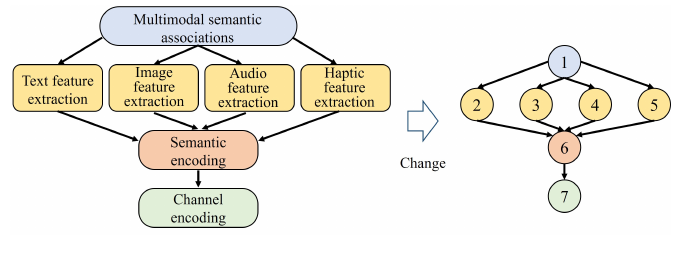
\includegraphics[width=0.8\linewidth]{fig/fig12.png}
\caption{적응성을 위한 ASC 구조 [154].}
\label{fig:12}
\end{figure}

최근의 최전선 에이전트 시스템은 빠른 추론 모드와 깊은 추론 모드 사이를 적응적으로 오가는 라우팅으로 오케스트레이션의 일부를 내재화한다. 한편 새로 등장하는 에이전트 프로토콜은 이종 에이전트 사이의 조정을 지원한다 [156]. ASC에서 이 변화는 적응성의 무게를 과업 스케줄링에서 에이전트 내부의 추론 제어와 에이전트 사이의 의미 조정으로 옮겨 놓는다. 그러나 동기화 오버헤드, 지연, 표준화 문제 때문에 ASC에 대규모 오케스트레이션을 도입하는 일은 여전히 과제로 남아 있다 [153], [157].

\subsubsection{창발적 통신을 통한 프로토콜 적응성}
ASC의 에이전트형 본질은 의미와 전략을 동적으로 조정하는 능력에 있다. 이 적응성은 창발적 통신(EmCom)/EmLang로 구현된다. 여기서 에이전트들은 사람의 개입 없이 에이전트 사이의 지속적인 상호작용을 통해 통신 프로토콜을 스스로 수립하고, 협상하고, 발전시킨다. 의미 통신 밖에서도 프로토콜 적응성은 더 넓은 네트워킹 연구계에서 오랫동안 연구되어 왔다. 예를 들어 DFG 공동연구센터 MAKI는 기능적으로 동등한 프로토콜 메커니즘 사이를 자동으로 전환해, 통신 시스템을 실행 중에 적응시키는 방법을 연구했다 [158]. 이와 달리 EmCom은 프로토콜 적응을 미리 정의된 메커니즘 가운데 하나를 고르는 일에서, 의미적 상호작용을 통해 통신 규칙을 적응적으로 수립하는 일로 확장한다.

AI 에이전트가 사람의 개입 없이 상호작용만으로 프로토콜을 수립할 수 있는지에 대해서는 대중의 관심도 컸다. 특히 ``코드로 소통하는 AI 에이전트''를 담은 영상이 널리 퍼졌는데, 이 영상은 새로운 기계 언어의 출현을 보여 주는 것으로 흔히 오해되었다 [159]. 그러나 실제로 이 영상이 보여 준 것은 GibberLink라는 미리 정의된 프로토콜의 사용이었다 [160]. 이것이 새로운 언어의 출현은 아니었지만, 대중의 반응은 AI 에이전트가 상호작용을 통해 통신 규칙을 만들어 낼 수 있는지에 대한 관심을 드러낸다.

EmLang의 개념적 연구는 Lewis의 신호 게임(signaling game)에 기반한 게임 이론적 틀에 뿌리를 둔다 [161]. 이 모형에서 송신자와 수신자는 신호--의미 관례를 반복적으로 형성하며, 명시적으로 합의하지 않고도 상호 이익을 최대화하는 체계로 수렴한다. 이후 딥러닝과 MARL이 발전하면서 이 신호 게임 패러다임은 신경망 기반 에이전트로 확장되었고, 통신 프로토콜을 자율적으로 형성할 수 있음이 입증되었다 [108].

이론적 실현 가능성은 최근 LLM을 이용한 실험으로 구체적으로 입증되었다. 연구자들 [162]은 무작위로 짝지은 AI 에이전트 24--200개에게 같은 대상에 이름을 붙이게 하는 실험을 했다. 같은 선택에는 보상을, 다른 선택에는 벌점을 주는 간단한 규칙만으로도 에이전트들은 몇 번의 상호작용 만에 공통 기호로 수렴했다. 이 결과는 프로토콜 수준에서 자율적 합의가 가능함을 시사한다. 그럼에도 이 실험은 신뢰할 수 있는 상호작용이라는 맥락에서 고정된 보상 규칙으로 제한되었다. 또한 구문 형성이나 오류 처리처럼 이름 붙이기를 넘어서는 프로토콜 기능은 고려하지 않았다. 구문 형성, 오류 복구, 개방형 환경에서의 상호 운용성 같은 더 복잡한 프로토콜 기능으로 확장할 수 있는지는 여전히 미해결 문제다.

자율적 합의라는 현상을 정식화하기 위해, EmLang·세계 모델·LLM을 잇는 생성적 틀로 집단 예측 부호화(CPC, collective predictive coding)가 제안되었다. CPC에 따르면 언어는 사회 집단 안에서 감각-운동 정보의 예측 가능성을 높이도록 진화했으며, 분산 베이즈 추론으로 모형화된다. 예를 들어 생성적 창발 통신(gEmCom, generative emergent communication) [163]은 CPC 가설에 기반한 생성 모델이다. 많은 EmLang 연구 [164], [165]는 판별적 모델링으로 통신 프로토콜을 최적화하는 데 집중해 왔다. 반면 CPC와 gEmCom은 언어의 출현을 생성 모델에 기반한 추론 과정으로 본다. 따라서 gEmCom 틀에서는 CPC가 언어를 생성하고, LLM은 그 언어로부터 집단 표현을 복원하는 복호기 역할을 한다.

\subsection{ASC의 다중 에이전트 기반 확장성}

\subsubsection{협력 통신과 조정}
ASC를 확장하면 다중 에이전트 통신이 필연적으로 뒤따르며, 이는 다중 에이전트 시스템(MAS) 환경에서 LLM 기반 기술의 발전을 이끈다. 이전의 MAS 연구는 규칙 기반 조정에 초점을 맞췄지만, LLM이 발전하면서 최근에는 자연어를 이용하는 MAS 연구들이 제안되었다.

LLM 에이전트 통신 연구들은 자연어를 넘어서는 공유 상태 표현이 협력 효율을 높일 수 있음을 보여 준다. 예를 들어 ChatDev [152]는 각 단계의 출력을 공유 메모리로 삼아 다음 단계로 넘긴다. 에이전트들이 중간 출력을 공유하면 공통 이해를 형성하고 맥락을 보존할 수 있다. 마찬가지로 Voyager [166]는 에이전트들을 위한 공유 KB 역할을 해, 한 에이전트가 학습한 의미 있는 지식을 다른 에이전트가 활용할 수 있게 하고, 이로써 경험의 공유를 돕는다.

ASC 시스템에서는 협력에 최적화된 공유 표현을 활용해 통신을 원활하게 하는 다양한 방법 [120], [167]--[169]이 제안되었다. 차량 네트워크에서 AI 에이전트는 시각-언어 모델을 이용해 원시 센서 데이터를 간결한 의미 표현으로 변환할 수 있다 [167]. 이 통합 방식은 이종 에이전트들 사이에 환경에 대한 공유된 이해를 촉진할 뿐 아니라, 대역폭 사용과 체감 품질(QoE, quality of experience) 사이의 절충도 최적화한다. 다중 에이전트 지각에서 PragCom은 시공간 희소화, 공유 부호책 압축, 피어 선택을 활용해 고정된 비트 예산 안에서 정확도를 최적화한다 [168]. EmCom에 기반한 협력 방식도 제안되었는데 [120], 여기서 에이전트들은 특정 과업을 풀기 위한 통신 프로토콜을 독립적으로 만들어 낸다. 더 나아가 여러 에이전트에게 통일된 KB가 없다는 문제를 해결하기 위해 명명 게임(naming game)을 활용한 연구가 제안되었다 [169]. 그림~\ref{fig:13}은 MAS의 ASC 구조와 에이전트 사이의 명명 게임 과정을 보여 준다. 이러한 연구들은 잠재 표현을 공유해 협력을 강화하지만, 에이전트들 사이의 합의가 해석 가능성을 해칠 수 있다. 따라서 이종·대규모 환경에서 신뢰할 수 있는 협력을 보장하려면 해석 가능한 표현 학습을 함께 도입해야 한다.

\setcounter{figure}{12}
\begin{figure}[htbp]
\centering
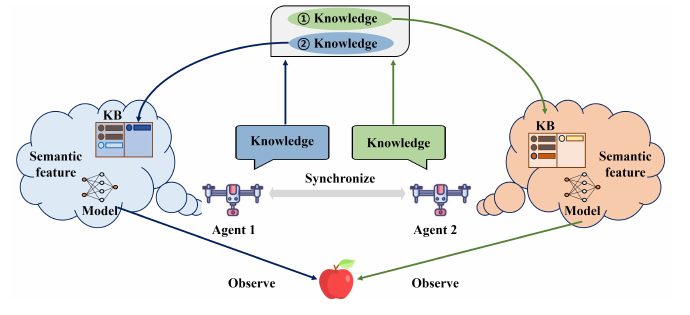
\includegraphics[width=0.8\linewidth]{fig/fig13.png}
\caption{MAS를 위한 ASC 구조 [169].}
\label{fig:13}
\end{figure}

구조화된 데이터를 공유 상태로 활용하는 연구들 [170]--[172]도 제안되었다. 한 연구 [170]에서는 LLM을 공유 KB로 써서 복잡한 데이터를 분할 지도와 경계 상자 같은 구조화된 의미 표현으로 변환하고, 이를 공유해 다중 사용자 협력에 활용했다. [171]에서는 센서가 환경 관측을 공유 격자 세계 지도에 갱신하고, 로봇은 이 지도를 이용해 과업을 수행한다. 화자와 청자가 계층적 신념 집합(hierarchical belief set)이라는 공통 언어로 협력하는 모델도 제안되었다 [172]. 이 모델에서는 단순한 문장 대신 여러 수준으로 추상화된 신념으로 이루어진 구조화된 표현 덕분에 정보를 더 효율적으로 전달할 수 있다. 구조화된 의미 표현을 활용하면 대화형 데이터를 쓸 때보다 과업 관련 정보를 더 효율적으로 교환할 수 있다는 점이 두드러진 장점이다.

\subsubsection{엣지 배포 전략}
AI 기반 네트워크에서는 다층 구조를 구축하기 위해 엣지--클라우드 협력이 구상되어 왔다 [170]. 그러나 자원이 제약된 환경에 에이전트를 배포하는 데에는 계산 능력과 에너지 소비에 관련된 어려움이 따른다. 따라서 이러한 제약 아래에서 동작하려면 ASC 에이전트를 경량화된 형태나 오프로딩되는 형태로 설계해야 한다 [173], [174].

경량 구조는 가지치기, 양자화, 지식 증류를 통해 과업 성능을 유지하면서 모델 복잡도를 줄인다 [173]--[175]. 또한 설계 단계부터 소형 구조를 채택하면 추론 효율을 높일 수 있다. 시스템 1과 시스템 2를 결합한 경량 LLM에 관한 최근 연구 [176]는 과업에 최적화된 초소형 LLM이 기존 구조보다 모델 크기를 크게 줄이면서도 성능을 높일 수 있음을 보여 준다. 이 결과는 ASC 프레임워크가 소규모 LLM으로도 계산 효율과 과업 지향 성능을 달성할 수 있음을 입증한다.

계산 오프로딩은 에이전트 추론을 엣지--클라우드 계층에 분산하는 수단으로 연구되어 왔다 [170]. 모델 분할은 신경망 층을 로컬 기기와 엣지 서버로 나눈다. 이와 달리 시간 분할 복호는 초기 반복을 엣지에서 실행하고 최종 정제는 로컬에서 마무리함으로써, 생성 모델의 부분 오프로딩을 가능하게 한다.

데이터 효율은 과업과 관련된 정보만 선택적으로 전송해 얻는다. 에이전트는 부분 의미 샘플링으로 과업과 관련된 데이터 조각을 전송하고, 수신 측은 이 조각들을 합쳐 과업 지향 복원을 수행한다 [175]. [177]에서는 정보 이득에 따라 의미적으로 중요한 토큰을 선택적으로 보존하는 놀람(surprisal) 유도 압축이 제안되었다. 이 압축을 LLM 기반 에이전트에 적용하면 전송 지연과 에너지 소비를 크게 줄일 수 있다. 모듈형 계층 설계는 과업을 전문화된 에이전트들로 분해한다 [178]. 상위 에이전트는 장기 목표를 다루고, 하위 에이전트는 채널 상태에 맞춰 의미 압축을 조정한다 [178].

\subsection{6G 네트워크에서의 ASC 구현}

\subsubsection{ASC 학습 파이프라인}
앞의 소절들에서는 ASC의 기본 능력들을 소개했다. 이 소절에서는 이를 세 단계로 이루어진 학습 파이프라인으로 묶는다. 세 단계는 (i) MARL 기반 ASC 학습, (ii) OOD 강건성을 위한 세계 모델 시뮬레이션, (iii) 적응적 추론 제어다.

\paragraph{a) MARL 기반 ASC 학습}
첫 단계는 MARL을 통해 ASC 에이전트의 기본 정책을 확립한다. 협력하는 에이전트 $N$개의 집합을 생각하자. 각 에이전트 $i$는 국소 정책 $\pi_{\theta_i}(a_i \mid o_i)$를 유지한다. 이 정책은 에이전트의 국소 관측 $o_i$(예: 원천 데이터의 의미 특징이나 추정된 CSI)를 행동 $a_i$(예: 의미 압축률, 부호책 선택, 전송 여부 결정)로 사상한다.

기존의 비트 수준 목표와 달리, ASC는 과업 수준의 의미 보상을 최적화한다. 시간 단계 $t$에서 각 에이전트의 보상은 다음과 같이 정식화할 수 있다.
\begin{equation}
R_t^i = r_{\mathrm{local}}^i(o_i, a_i) + R_{\mathrm{cluster}}(\bm{\tau}, \mathbf{a}) - c_i(o_i, a_i), \tag{7}
\end{equation}
여기서 $\mathbf{a} = (a_1, \ldots, a_N)$은 결합 행동이고, $\bm{\tau} = (\tau_1, \ldots, \tau_N)$은 결합 행동-관측 이력이다. 하류 의미 과업에 대한 각 에이전트의 개별 기여는 $r_{\mathrm{local}}^i$로 정량화하고, $c_i$는 에이전트의 전송 오버헤드다. $R_{\mathrm{cluster}}$는 협력 과업 성능을 반영하며, 에이전트들이 자신의 표현을 공유 프로토콜에 정렬하도록 유도한다. 이로써 명시적인 지도 없이도 과업에 최적화된 통신 언어가 창발한다.

6G의 대규모 엣지 환경을 고려하면, 중앙집중 학습·분산 실행(CTDE, centralized training with decentralized execution)이 적절한 선택이다. 이 틀을 지원하기 위해, 다중 에이전트 학습에서 확장성과 안정성을 갖춘 다중 에이전트 근접 정책 최적화(MAPPO, multi-agent proximity policy optimization)\onote{MAPPO의 원래 명칭은 multi-agent \emph{proximal} policy optimization이다.}를 구현한다. MAPPO는 전역 상태 $s$에서 평가되는 중앙집중 비평자 네트워크 $V_\phi(s)$를 쓴다. 분산된 각 행위자는 다음의 절단 대리 목적함수(clipped surrogate objective)를 최대화하도록 자신의 정책을 갱신한다.
\begin{equation}
L(\theta_i) = \E\Big[\min\Big(\rho_i \hat{A}_i,\, \mathrm{clip}(\rho_i, 1-\epsilon, 1+\epsilon)\hat{A}_i\Big)\Big], \tag{8}
\end{equation}
여기서 $\rho_i$는 정책 비율이고, $\hat{A}_i$는 중앙집중 비평자가 추정한 어드밴티지다.

\paragraph{b) OOD 강건성을 위한 세계 모델 시뮬레이션}
OOD 상황에서 모델의 강건성을 높이기 위해 세계 모델을 쓴다. 이 모델은 MARL 학습 과정에서 얻은 궤적을 바탕으로 환경의 동역학을 예측하도록 구축된다. 환경으로부터 동역학을 학습한 세계 모델은 동적 계획 과정 $H$에 걸쳐 합성 롤아웃을 생성할 수 있다. 또한 세계 모델은 송신기에서 추상화 모듈 역할도 한다. 즉 원시 고차원 관측을 그대로 전송하는 대신, 다중 모달 입력을 간결한 의미 잠재 상태로 부호화한다.

각 에이전트는 합성 궤적을 이용해 다음과 같이 정책을 갱신한다.
\begin{equation}
\theta_i \leftarrow \theta_i + \alpha\, \nabla_{\theta_i} \E_{\hat{T},\, \pi_{\theta_i}}\left[\sum_{\tau=t}^{t+H} \gamma^{\tau-t} \hat{R}(\hat{s}_\tau, \hat{a}_\tau)\right], \tag{9}
\end{equation}
여기서 $\alpha$는 학습률이고 $\gamma$는 할인 인자다. 이 모델 기반 갱신 덕분에 에이전트는 원래라면 대규모 탐색이 필요했을 일반화 능력을 얻을 수 있다 [43]. 모델은 또한 분포 불일치의 정도를 반영하는 예측 오차 $\epsilon_t$(V-A6절에서 정의)를 출력한다. $\epsilon_t < \epsilon_{\mathrm{th}}$이면 수신기의 세계 모델이 과업 수행에 충분한 의미 충실도를 유지하므로 전송을 건너뛸 수 있다. 그렇지 않으면 재계획이나 전송을 실행한다 [116].

\paragraph{c) 적응적 추론 제어}
배포 단계에서 에이전트는 실시간 지연·에너지 예산 안에서 동작해야 한다. 이 요구를 충족하기 위해, ASC의 마지막 단계는 시스템 1/시스템 2 틀 [35]에서 착안한 이중 모드 추론 메커니즘을 쓴다. 시스템 1은 과업에 최적화된 소형 LLM이나 MARL 정책에 의존해 일상적인 통신 과업을 처리한다. 시스템 2는 복잡하거나 낯선 상황에서 세계 모델 계획기와 함께 추론 파이프라인을 가동한다.

두 모드 사이의 전환은 (5)의 전환 변수가 제어하며, 이 변수는 (6)의 규칙을 따른다. 예측 오차 $\epsilon_t$는 현재 관측이 얼마나 예상 밖인지를 정량화하는 놀람 신호로 해석할 수 있고, 따라서 에이전트의 토큰화와 전송 결정을 내리는 데 도움을 준다. 에이전트는 기본적으로 시스템 1을 쓰고 필요할 때만 시스템 2를 호출함으로써, 과업 성능을 유지하면서 추론 지연과 에너지 소비를 줄인다.

6G 구조에서 이 세 단계는, O-RAN 기반 배포의 한 후보로서, II절에서 설명한 RIC 제어 계층에 대응시킬 수 있다. MARL 기반 학습과 세계 모델 학습은 비실시간 RIC에 rApp으로 배치하며, 그 제어 루프는 1초보다 긴 간격으로 동작한다. 반면 적응적 추론 제어는 준실시간 RIC에서 xApp으로 실행하며, 그 제어 루프는 10~ms에서 1~s 정도의 간격으로 동작한다 [179]. 시스템 2 추론이 이 예산을 넘기면, 현재 결정은 시스템 1이 내리고 시스템 2의 결과는 나중에 비동기 정책 갱신으로 반영한다. 이 대응은 경량 예측 제어기를 xApp으로 배포하고 LLM 기반 의도 변환기를 rApp으로 운용한 최근 구현 [28]과도 일치한다. 이렇게 얻은 정책과 모델 갱신은 비실시간 RIC에서 준실시간 RIC로 A1 인터페이스를 통해 전달되며, A1 인터페이스는 정책 관리와 ML 모델 관리 서비스를 제공한다 [179].

\subsubsection{ASC의 지원, 모니터링, 최적화}
앞서 설명한 O-RAN 대응은 ASC 기능을 배치하는 한 가지 방법을 보여 준다. 기능 배치를 넘어 ASC를 실현하려면 과업 인지 네트워크 지원, 모니터링, 폐루프 최적화가 필요하며, 이를 아래에서 논의한다. 이에 따라 6G 네트워크는 데이터 중심 자원 관리에서 통신·컴퓨팅·에이전트 상호작용의 과업 인지 오케스트레이션으로 진화해야 한다.

\paragraph{a) ASC 지원}
ASC는 과업 수준과 에이전트 수준의 정보를 고려함으로써 기존 네트워크 제어·관리를 확장한다. 3GPP TR 22.870은 AI 서비스와 AI 에이전트 사이의 통신을 위한 6G 활용 사례와 서비스 요구 사항을 다루며 [180], ITU-T 권고는 ML 파이프라인과 그 관리·오케스트레이션을 위한 구조적 틀을 제시한다 [181]. ASC에서는 의도, 의미 우선순위, 추론 마감 시한, 모델 또는 KB 식별자 같은 정보를 권한 있는 네트워크 제어 기능에 제공해 통신·컴퓨팅 자원 할당에 쓸 수 있다. 6G의 핵심 방향은 과업 의도와 에이전트 능력을 네트워크 제어에 반영해, 통신과 에이전트 상호작용을 과업 요구 사항에 따라 관리할 수 있게 하는 것이다.

\paragraph{b) ASC 모니터링}
네트워크 데이터 분석과 폐루프 제어 관리를 위한 기존 3GPP 메커니즘을 ASC 모니터링의 기반으로 적용할 수 있다 [182], [183]. 기존 네트워크 텔레메트리에 더해 과업 진행도, 추론 지연, 에이전트 가용성, 모델 또는 KB 일관성도 고려할 수 있다. 궁극적으로 ASC 모니터링은 네트워크 상태와 에이전트-과업 상태를 함께 볼 수 있게 해서, 통신 실패를 추론·지식·조정 실패와 구별할 수 있게 해야 한다.

\paragraph{c) ASC 최적화}
모니터링한 정보를 바탕으로, 네트워크 제어기와 에이전트 제어기는 폐루프 제어를 통해 통신, 계산, 에이전트 조정을 적응시킬 수 있다. 이에 해당하는 결정에는 전송과 스케줄링, 추론 배치, 피어 선택, 모델 또는 KB 동기화가 있다. 이러한 결정은 지연, 신뢰성, 에너지, 프라이버시, 컴퓨팅 제약을 고려하면서 과업 효용에 따라 최적화할 수 있다 [184]. 더 넓게 보면, ASC 제어는 통신·컴퓨팅·에이전트 상호작용이 바탕 과업의 진행과 성능에 기여하는 정도에 따라 이들을 조정해야 한다.

\subsubsection{ASC의 6G 프로토콜 스택 통합}
다음으로 6G 배포를 위해 알고리즘 수준의 통합에서 프로토콜 스택 수준의 통합으로 넘어간다. 의미 통신을 기존 계층형 스택에 통합하려는 최근 시도는 크게 두 방향에 집중해 왔다. 첫째 접근 [185], [186]은 호환성을 유지하기 위해 의미 통신 기능을 기존 프로토콜 스택에 대응시킨다. 둘째 접근 [187], [188]은 의미 추출, 맥락 추론, 과업 인식 최적화에 초점을 맞춰 계층 구조를 재설계한다. 구체적으로, 전자는 기존 PHY/MAC 스택을 수정하지 않고 전송 계층 위에 의미 기능을 둔다. 후자는 프로토콜 스택을 재구성해 전용 의미 계층을 도입한다. 이 서베이 전체에서 쓰는 계층 할당은 이 소절의 끝에서 설명한다.

프로토콜 스택의 하드웨어 교체 비용과 시스템 복잡도를 줄이기 위해, 개방형 시스템 상호 연결(OSI, open systems interconnection) 모델의 응용 계층 안에 의미 부계층을 결합하는 통합 방법이 제안되었다 [185]. 또한 기존 5세대(5G) 프로토콜 스택과 상호 운용되는 별도의 의미 기반(Seb, semantic-base) 프로토콜 스택도 제안되었다 [186]. 이러한 상호 운용형 접근은 기존 인프라와 점진적으로 통합하기 쉽게 해 주지만, 계층 간 처리 지연과 헤더 추가 때문에 오버헤드가 불가피하게 생긴다.

기존 프로토콜 스택을 의미 통신에 맞춘 3계층 모델로 재편한, 지능적이고 효율적인 의미 통신 구조가 제안되었다 [187]. Fleming 등은 OSI 모델에 새로운 계층 두 개를 추가할 것을 제안한다 [188]. 추가된 계층은 확장 가능한 분산 에이전트 협력의 토대가 되어, 차세대 통신 시스템을 가능하게 한다. 그러나 이러한 접근은 기존 레거시 시스템과의 상호 운용성을 잃을 수 있다.

표준화 관점에서 ASC는 진행 중인 3GPP 활동을 보완하는 통신 인지 오케스트레이션 계층으로 자리매김해야 한다. 최근 3GPP SA 논의는 다중 모달 토큰 스트림과 GAI 기반 서비스를 부각한다 [104], [180]. 그러나 의미적 의도 협상, 에이전트 간 맥락 정렬, 분산 도구 오케스트레이션, 토큰 수준 조정은 아직 명시적으로 표준화되지 않았다. 이러한 공백은 ASC를 실제로 배포하기 쉽게 하려면 AI/ML 모델 관리, 에이전트 조정, 그리고 이종 클라우드--엣지--기기 개체에 걸친 추론 배치를 표준화된 방식으로 지원해야 함을 보여 준다. 이에 따라 그림~\ref{fig:14}에 나타낸 것처럼, ASC는 프로토콜 스택 전반에서 토큰 중심 처리를 가능하게 하는 호환 가능한 에이전트형 평면(Agentic Plane)으로 해석된다. 응용 계층에서는 사용자 에이전트(User Agent)가 LLM과 의미 KB를 활용해 과업 지향 의도를 생성한다. 네트워크 계층에서는 에이전트형 제어기(Agentic Controller)가 세계 모델과 보조 모듈을 이용해 선제적 정책을 수립한다. 데이터 링크 계층의 에이전트형 스케줄러(Agentic Scheduler)는 우선순위를 고려한 스케줄링을 결정한다. PHY 계층에서는 에이전트형 송수신기(Agentic Transceiver)가 기존 모듈과 공존하면서 의미 심볼을 처리하고, 에이전트의 의도를 ASC 인프라로 전달한다.

\setcounter{figure}{13}
\begin{figure}[htbp]
\centering
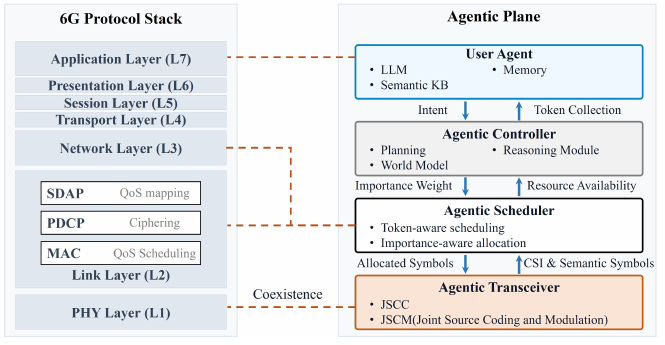
\includegraphics[width=0.85\linewidth]{fig/fig14.png}
\caption{6G 프로토콜과 그에 정렬된 스택.}
\label{fig:14}
\end{figure}

\subsubsection{ASC의 디지털 호환성}
직관 기반 의미 통신의 디지털 호환성은 주로 심볼 수준의 문제다. 반면 ASC는 여기에 더해 토큰 수준과 프로토콜 수준의 호환성도 요구한다. 의미 토큰은 이산 인덱스로 표현되므로 비트열로 대응시켜 기존 변조, 채널 부호화, 패킷화로 전송할 수 있다 [102]. 패킷화는 패킷 손실의 영향을 국한하고, 재전송 시에는 의미적으로 중요한 토큰을 우선할 수 있다 [103]. 또한 세계 모델 기반 건너뛰기 절차는 수신기가 자신의 세계 모델로 추론할 수 있는 토큰을 생략한다. 이로써 트래픽 수요가 줄고, MAC 스케줄러는 확보된 자원을 다른 사용자에게 할당할 수 있다 [116]. 프로토콜 수준에서 EmLang은 공유 토큰 부호책을 필요로 하며, 부호책 갱신 메커니즘과 프로토콜 수렴에 실패했을 때 미리 정의된 어휘로 되돌아가는 대체 메커니즘도 함께 갖춰야 한다(V-C절). 이어서 에이전트형 스케줄링이 무엇을 언제 전송할지 결정하고 (3)의 자원 요청 $\rho_{ij}^t$를 발행한다. 이 요청은 의미 우선순위, 마감 시한, 허용 왜곡 같은 속성을 지정하며, 하위 PHY/MAC 계층은 이 요청을 자원 블록과 변조·부호화 방식 같은 물리 무선 자원에 대응시킨다 [179].

\subsection{선행 연구에서 얻은 교훈}
최근 ASC 연구 전반에 걸친 핵심 변화는 고정된 통신 파이프라인에서 폐루프 의미 제어로의 전환이다. ASC 에이전트는 의미 표현을 전송하는 데서 나아가, 무엇을 전송할지, 언제 추론할지, 자신의 행동을 어떻게 수정할지를 스스로 결정하는 방향으로 진화하고 있다. 이 능력을 갖추기 위해 최근 연구들은 LLM 기반 프레임워크 안에 계획, 메모리, 자기 교정, 검색, 작업 흐름 오케스트레이션을 통합해 왔다.

ASC의 주된 과제는 안정성, 효율성, 효과성 사이의 균형이다. 세계 모델은 계획을 지원하고, 메모리는 맥락을 보존하며, RAG는 결정의 신뢰성을 높인다. EmCom 기반 방법과 NeSy 기반 방법은 조정 문제를 다루고, 자기 교정은 실행 오류를 완화한다. 이러한 메커니즘을 통해 맥락이 바뀔 때 에이전트의 행동을 조정할 수 있다. 다중 에이전트 환경에서 최근 연구들은 주로 계산 오프로딩, 경량 배포, 모듈형 설계, 구조화된 상태 교환에 초점을 맞춰 왔다. 전반적으로 ASC 구현은 대체로 자원 인지 오케스트레이션의 문제로 다뤄져 왔다. 표~\ref{tab:9}에 관련 문헌을 정리했다.

\setcounter{table}{8}
\begin{table}[htbp]
\centering
\caption{ASC 문헌 검토}
\label{tab:9}
\footnotesize
\renewcommand{\arraystretch}{1.25}\renewcommand{\tabularxcolumn}[1]{m{#1}}
\begin{tabularx}{\linewidth}{>{\centering\arraybackslash}m{0.24\linewidth}|>{\centering\arraybackslash}m{0.13\linewidth}|>{\centering\arraybackslash}X}
\hline
\textbf{핵심 능력} & \textbf{참고문헌} & \textbf{특징} \\
\hline
자율성(예측 계획) & [115], [116], [122]--[125] & 보상 유도 미래 상태 예측, 의미 추상화, 예측 오차에 기반한 전송 건너뛰기를 위한 내부 세계 모델 \\
\hline
자율성(동적 계획) & [37], [129]--[131] & 사용자 의도를 하위 과업으로 분해하고, 빠른 실행과 더 깊은 추론 사이에서 추론 깊이를 조정하는 계획 및 계획기-실행기 프레임워크 \\
\hline
\multirow{2}{=}{\centering 자율성(도구 사용)} & [132]--[136], [139] & 외부 지식에 결정을 근거 지어 환각을 줄이고 신뢰성을 높이는 검색·도구 증강 프레임워크 \\
\cline{2-3}
 & [137] & 통신에서 RAG를 보완하기 위한 보안 전략 \\
\hline
자율성(메모리) & [117], [140]--[143] & 맥락, 이력, 환경을 저장해 맥락 이해와 전송 효율을 높이는 메모리 모듈 \\
\hline
자율성(자기 교정) & [119], [148] & 에이전트가 의미 오류를 자율적으로 탐지·교정할 수 있게 하는 프레임워크 \\
\hline
적응성(운영) & [154], [155] & 성능과 자원 효율의 균형을 맞추며 과업을 관리하는 오케스트레이션 프레임워크 \\
\hline
적응성(프로토콜) & [108], [162]--[165] & 반복적인 상호작용을 통해 에이전트가 공유 통신 프로토콜을 자율적으로 발전시키고 그 프로토콜로 수렴하게 하는 방법 \\
\hline
\multirow{2}{=}{\centering 다중 에이전트 시스템\\(협력)} & [120], [167]--[169] & 자연어 대신 암묵적 공유 표현을 통한 협력 \\
\cline{2-3}
 & [152], [166], [170]--[172] & 공통 이해를 위해 명시적 공유 상태(구조화된 데이터, 메모리, KB)를 이용한 조정 \\
\hline
\multirow{4}{=}{\centering 다중 에이전트 시스템\\(엣지 배포)} & [173]--[176] & 경량화 기법을 이용한 모델 복잡도 감소 \\
\cline{2-3}
 & [170] & 효율적 추론을 위한 계산 오프로딩 활용 \\
\cline{2-3}
 & [175], [177] & 선택적 전송과 놀람 유도 압축을 통한 개별 에이전트의 통신 부하 감소 \\
\cline{2-3}
 & [178] & 시스템 복잡도를 줄이기 위한 모듈형 계층 에이전트 설계 \\
\hline
\end{tabularx}
\end{table}

이러한 관찰에서 세 가지 핵심 통찰을 끌어낼 수 있다. 첫째, 자율성은 LLM의 추론 능력이 아니라, 과업 맥락과 자원 상태에 따라 적응적으로 의사 결정을 할 수 있게 하는 제어 능력으로 이해해야 한다. 따라서 ASC의 핵심은 모듈들을 통합해 폐루프 의사 결정 과정을 확립하는 데 있다. 둘째, 의미는 지속적으로 검증되고 수정될 때에만 신뢰할 수 있다. 따라서 의미 표류와 불안정한 협력을 막으려면 되먹임, 예측, 조정 신호를 통해 의미를 검증해야 한다. 셋째, ASC의 확장성은 모델 크기만으로 정해지지 않는다. 확장성은 모델 복잡도, 조정 위상, 동기화 오버헤드, 추론 배치에 함께 좌우된다. 에이전트 수가 늘어나면, 성능은 추론 깊이, 계산 배치, 조정 위상 같은 모듈을 자원 제약 아래에서 얼마나 효율적으로 제어하느냐에 달려 있다. 예를 들어 에이전트 수백 개가 한 셀을 공유한다면, 모델 크기를 키우는 것만으로는 조정 트래픽이나 동기화 지연을 줄일 수 없다. 이때 시스템 성능은 어떤 에이전트가 깊은 추론을 호출하는지, 추론이 기기·엣지·클라우드에 걸쳐 어떤 방식으로 실행되는지, 에이전트들이 메시지를 어떻게 교환하는지에 달려 있다. 따라서 ASC의 발전은 견고한 추론을 수행하는 에이전트를 만드는 일보다, 분산된 에이전트들 사이에서 의미적 일관성을 어떻게 유지할지 정하는 구조에 더 크게 좌우될 것이다.

\setcounter{table}{9}
\begin{table}[htbp]
\centering
\caption{의미 통신 및 에이전트형 통신 시스템의 평가 지표}
\label{tab:10}
\footnotesize
\renewcommand{\arraystretch}{1.25}\renewcommand{\tabularxcolumn}[1]{m{#1}}
\begin{tabularx}{\linewidth}{>{\centering\arraybackslash}m{0.12\linewidth}|>{\centering\arraybackslash}m{0.13\linewidth}|>{\centering\arraybackslash}m{0.14\linewidth}|>{\centering\arraybackslash}X|>{\centering\arraybackslash}m{0.22\linewidth}}
\hline
\textbf{평가 범위} & \textbf{모달리티 / 대상} & \textbf{평가 단위} & \textbf{대표 지표} & \textbf{평가 대상} \\
\hline
\multirow{4}{=}{\centering 모달리티별} & 텍스트 & 문장, 문서 & BLEU, BERTScore, MoverScore, BLEURT, COMET, BARTScore & 표면 형태와 의미의 보존 \\
\cline{2-5}
 & 음성 & 발화 & PESQ, WER/CER, SpeechBERTScore, SeMaScore & 지각 품질, 전사 정확도, 또는 의미 보존 \\
\cline{2-5}
 & 이미지, 비디오 & 이미지/프레임, 비디오 집합 & PSNR, SSIM, LPIPS, SeSS, ViTScore, FVD & 화소, 지각, 의미, 또는 시공간 분포 충실도 \\
\cline{2-5}
 & 3D 점구름, 시계열 센서 & 점구름, 시계열 & Chamfer 거리, RMSE, DTW & 기하적 또는 시간적 충실도 \\
\hline
교차 모달 정렬 & 다중 모달 & 짝지은 표본, 검색 집합 & CLIPScore, CLAP 유사도, ImageBind 유사도, Recall@K & 교차 모달 의미 정렬 \\
\hline
과업 효과성 & 과업 실행 & 에피소드, 에이전트 팀 & TSP, ToD, 지연--과업 보상 곡선, 에이전트--과업 효용 & 과업 완수, 출력 품질, 성능 절충 \\
\hline
시스템 효율 & 통신과 계산 & 종단 간 시스템, 과업 설정 & 비트 수, 채널 사용 횟수, FLOPs, 지연, 에너지 & 자원 비용, 그리고 그 비용과 의미·과업 효과성의 관계 \\
\hline
\end{tabularx}
\end{table}
